\documentclass[11pt]{amsart}
\usepackage{geometry}                % See geometry.pdf to learn the layout options. There are lots.
\geometry{letterpaper}                   % ... or a4paper or a5paper or ... 
%\geometry{landscape}                % Activate for for rotated page geometry
%\usepackage[parfill]{parskip}    % Activate to begin paragraphs with an empty line rather than an indent
\usepackage{graphicx}
\usepackage{amssymb}
\usepackage{epstopdf}
\usepackage{hyperref}
\usepackage{/Library/Frameworks/R.framework/Resources/share/texmf/Sweave}
\DeclareGraphicsRule{.tif}{png}{.png}{`convert #1 `dirname #1`/`basename #1 .tif`.png}

\title{Solidago Flower Arthropod Network Modeling and Analyses}
\author{M.K. Lau}
\date{}                                           % Activate to display a given date or no date

\begin{document}
\maketitle

\setcounter{tocdepth}{3}
\tableofcontents


\subsection*{Network Modelling Summary}
\begin{enumerate}
\item Species with abundances of two or less were removed (see
  \hyperlink{rm.s&d}{above})
\item The data were separated into two graphs, \textbf{Elk} and \textbf{No Elk}
  exposure
\item The p-values for the correlation tests were not corrected for
  experimentwise error
\end{enumerate}


\subsection*{Meta-Data}
\begin{itemize}
\item Solidago Pollinator Network Analyses
\item Project Director: Dave Smith
\item Data Recorder: Ryan ? (undergrad assistant)
\item NOTE FROM DAVE ABOUT PREVIOUS ANALYSES: I did not include population FS in my analysis for elk / no-elk.  Although, they could be useful data for looking at heritability or perhaps something else.  Also, for my analysis, I only included families with more than one rep (I also did an analysis including only families with 3 or more reps).  And, I removed singletons from the data.
\end{itemize}



\section{Analyses and Figures}
\subsection{Package Dependencies}


%%Check if igraph is loaded and remove if needed
\begin{Schunk}
\begin{Soutput}
NULL
\end{Soutput}
\end{Schunk}

\begin{Schunk}
\begin{Sinput}
> require(ecodist)
> require(sna)
\end{Sinput}
\begin{Soutput}
     Tools for Social Network Analysis
Version      2.2-0 created on      2010-11-21.
copyright (c) 2005, Carter T. Butts, University of California-Irvine
Type help(package="sna") to get started.
\end{Soutput}
\begin{Sinput}
> require(vegan)
> require(xtable)
> source("/Users/Aeolus/Documents/Active_Projects/CorNets/CorNets.R")
\end{Sinput}
\end{Schunk}

\begin{Schunk}
\begin{Sinput}
> bin.sum = function(x) {
+     x[x != 0] = 1
+     sum(x)
+ }
\end{Sinput}
\end{Schunk}

\subsection{Data Summary}

\begin{Schunk}
\begin{Sinput}
> data = read.csv("SolidagoPollinators2010.csv")
> summary(data)
\end{Sinput}
\begin{Soutput}
      Family      Individual   RandomNmbr          Population  Elk.   
 FS 16   : 14   A      :38   Min.   :0.0001008   FS     :51      :51  
 Kiwi 10 : 13   B      :30   1st Qu.:0.2579153   Ft Vall:26   No :65  
 FS 18   : 11   C      :25   Median :0.5235663   Grnhs  :21   Yes:96  
 Grnhs 10:  9   D      :21   Mean   :0.5124183   K In   :30           
 Kiwi 28 :  9   E      :16   3rd Qu.:0.7546771   K Out  :31           
 FS 22   :  8   F      :14   Max.   :0.9986857   Keeli  :39           
 (Other) :148   (Other):68                       Thorpe :14           
               Notes       Florettes      Flors.per.stalk   Date.of.Flwr   
                  :208   Min.   :  7.00   Min.   :  2.25   Min.   :  1.00  
 only 1 srvy date?:  1   1st Qu.: 37.00   1st Qu.: 18.65   1st Qu.: 67.00  
 only 1 survey    :  1   Median : 65.50   Median : 32.67   Median : 77.00  
 only 2 survey    :  1   Mean   : 78.05   Mean   : 46.51   Mean   : 77.57  
 Only one sample? :  1   3rd Qu.: 96.25   3rd Qu.: 66.62   3rd Qu.: 91.00  
                         Max.   :281.00   Max.   :227.00   Max.   :113.00  
                                                                           
  Date.of.Srvy    Total.Height.mm.     Stalks          Ramets      
 Min.   : 65.00   Min.   :107.0    Min.   :1.000   Min.   :0.0000  
 1st Qu.: 66.25   1st Qu.:290.2    1st Qu.:1.000   1st Qu.:0.0000  
 Median : 67.50   Median :342.0    Median :2.000   Median :0.0000  
 Mean   : 67.50   Mean   :344.2    Mean   :2.146   Mean   :0.1604  
 3rd Qu.: 68.75   3rd Qu.:395.8    3rd Qu.:3.000   3rd Qu.:0.0000  
 Max.   : 70.00   Max.   :586.0    Max.   :6.000   Max.   :3.0000  
 NA's   :210.00   NA's   :  2.0                                    
  Grey.Beetle         Aphid             Ant         BlackOrangeWasp 
 Min.   : 0.000   Min.   :  0.00   Min.   :0.0000   Min.   :0.0000  
 1st Qu.: 0.750   1st Qu.:  0.00   1st Qu.:0.0000   1st Qu.:0.0000  
 Median : 3.000   Median :  4.00   Median :0.0000   Median :0.0000  
 Mean   : 8.476   Mean   : 13.89   Mean   :0.2877   Mean   :0.0566  
 3rd Qu.:10.000   3rd Qu.: 16.00   3rd Qu.:0.0000   3rd Qu.:0.0000  
 Max.   :79.000   Max.   :174.00   Max.   :4.0000   Max.   :3.0000  
                                                                    
  Syrphid.Fly      RedBlackFly      LargeHairyFly        Tiny.Fly      
 Min.   :0.0000   Min.   :0.00000   Min.   :0.00000   Min.   : 0.0000  
 1st Qu.:0.0000   1st Qu.:0.00000   1st Qu.:0.00000   1st Qu.: 0.0000  
 Median :0.0000   Median :0.00000   Median :0.00000   Median : 0.0000  
 Mean   :0.2075   Mean   :0.03302   Mean   :0.02358   Mean   : 0.6085  
 3rd Qu.:0.0000   3rd Qu.:0.00000   3rd Qu.:0.00000   3rd Qu.: 1.0000  
 Max.   :8.0000   Max.   :2.00000   Max.   :2.00000   Max.   :11.0000  
                                                                       
  GreenTrueBug     SkinnyBlackFly    BlackYellowFly    TinyRedSpider     
 Min.   :0.00000   Min.   :0.00000   Min.   :0.00000   Min.   :0.000000  
 1st Qu.:0.00000   1st Qu.:0.00000   1st Qu.:0.00000   1st Qu.:0.000000  
 Median :0.00000   Median :0.00000   Median :0.00000   Median :0.000000  
 Mean   :0.02358   Mean   :0.08962   Mean   :0.01415   Mean   :0.009434  
 3rd Qu.:0.00000   3rd Qu.:0.00000   3rd Qu.:0.00000   3rd Qu.:0.000000  
 Max.   :1.00000   Max.   :3.00000   Max.   :2.00000   Max.   :1.000000  
                                                                         
 BrightGreenFly      GreyMoth         BlackWasp          GreyFly        
 Min.   :0.0000   Min.   :0.00000   Min.   :0.00000   Min.   :0.000000  
 1st Qu.:0.0000   1st Qu.:0.00000   1st Qu.:0.00000   1st Qu.:0.000000  
 Median :0.0000   Median :0.00000   Median :0.00000   Median :0.000000  
 Mean   :0.0283   Mean   :0.01415   Mean   :0.01887   Mean   :0.004717  
 3rd Qu.:0.0000   3rd Qu.:0.00000   3rd Qu.:0.00000   3rd Qu.:0.000000  
 Max.   :3.0000   Max.   :2.00000   Max.   :1.00000   Max.   :1.000000  
                                                                        
 MaroonHorseFly          Wasp          HumpbackFly          Thrips       
 Min.   :0.000000   Min.   :0.00000   Min.   :0.00000   Min.   :0.00000  
 1st Qu.:0.000000   1st Qu.:0.00000   1st Qu.:0.00000   1st Qu.:0.00000  
 Median :0.000000   Median :0.00000   Median :0.00000   Median :0.00000  
 Mean   :0.004717   Mean   :0.06132   Mean   :0.04717   Mean   :0.03302  
 3rd Qu.:0.000000   3rd Qu.:0.00000   3rd Qu.:0.00000   3rd Qu.:0.00000  
 Max.   :1.000000   Max.   :1.00000   Max.   :4.00000   Max.   :3.00000  
                                                                         
   SkinnyBee          FruitFly           BrownFly          HoneyBee      
 Min.   :0.00000   Min.   :0.000000   Min.   :0.00000   Min.   :0.00000  
 1st Qu.:0.00000   1st Qu.:0.000000   1st Qu.:0.00000   1st Qu.:0.00000  
 Median :0.00000   Median :0.000000   Median :0.00000   Median :0.00000  
 Mean   :0.01887   Mean   :0.009434   Mean   :0.01887   Mean   :0.08019  
 3rd Qu.:0.00000   3rd Qu.:0.000000   3rd Qu.:0.00000   3rd Qu.:0.00000  
 Max.   :2.00000   Max.   :1.000000   Max.   :1.00000   Max.   :4.00000  
                                                                         
 BrightGreenBee      BigBlackFly       BlackGreyFly     SkinnyBlackBee
 Min.   :0.000000   Min.   :0.00000   Min.   :0.00000   Min.   :0     
 1st Qu.:0.000000   1st Qu.:0.00000   1st Qu.:0.00000   1st Qu.:0     
 Median :0.000000   Median :0.00000   Median :0.00000   Median :0     
 Mean   :0.004717   Mean   :0.04245   Mean   :0.08019   Mean   :0     
 3rd Qu.:0.000000   3rd Qu.:0.00000   3rd Qu.:0.00000   3rd Qu.:0     
 Max.   :1.000000   Max.   :3.00000   Max.   :3.00000   Max.   :0     
                                                                      
 Microbutterfly    LongHornBeetle    RedThoraxBeetle      RedGreyFly      
 Min.   :0.00000   Min.   :0.00000   Min.   :0.000000   Min.   :0.000000  
 1st Qu.:0.00000   1st Qu.:0.00000   1st Qu.:0.000000   1st Qu.:0.000000  
 Median :0.00000   Median :0.00000   Median :0.000000   Median :0.000000  
 Mean   :0.01887   Mean   :0.03774   Mean   :0.004717   Mean   :0.004717  
 3rd Qu.:0.00000   3rd Qu.:0.00000   3rd Qu.:0.000000   3rd Qu.:0.000000  
 Max.   :1.00000   Max.   :2.00000   Max.   :1.000000   Max.   :1.000000  
                                                                          
  Caterpillar       BrightGreenSpider  SkinnyBrownSpider  BlackWhiteFly    
 Min.   :0.000000   Min.   :0.000000   Min.   :0.000000   Min.   :0.00000  
 1st Qu.:0.000000   1st Qu.:0.000000   1st Qu.:0.000000   1st Qu.:0.00000  
 Median :0.000000   Median :0.000000   Median :0.000000   Median :0.00000  
 Mean   :0.004717   Mean   :0.009434   Mean   :0.009434   Mean   :0.02358  
 3rd Qu.:0.000000   3rd Qu.:0.000000   3rd Qu.:0.000000   3rd Qu.:0.00000  
 Max.   :1.000000   Max.   :1.000000   Max.   :1.000000   Max.   :3.00000  
                                                                           
   Robber.Fly       OrangeYellowHairyBee MetallicBlueFly       Ladybug        
 Min.   :0.000000   Min.   :0.0000       Min.   :0.000000   Min.   :0.000000  
 1st Qu.:0.000000   1st Qu.:0.0000       1st Qu.:0.000000   1st Qu.:0.000000  
 Median :0.000000   Median :0.0000       Median :0.000000   Median :0.000000  
 Mean   :0.004717   Mean   :0.0283       Mean   :0.004717   Mean   :0.004717  
 3rd Qu.:0.000000   3rd Qu.:0.0000       3rd Qu.:0.000000   3rd Qu.:0.000000  
 Max.   :1.000000   Max.   :2.0000       Max.   :1.000000   Max.   :1.000000  
                                                                              
 BlackOrangeButterfly OrangeAbdomenFly   GreenCaterpillar   OrangeAbdomenFly.1
 Min.   :0.000000     Min.   :0.000000   Min.   :0.000000   Min.   :0.000000  
 1st Qu.:0.000000     1st Qu.:0.000000   1st Qu.:0.000000   1st Qu.:0.000000  
 Median :0.000000     Median :0.000000   Median :0.000000   Median :0.000000  
 Mean   :0.009434     Mean   :0.004717   Mean   :0.004717   Mean   :0.004717  
 3rd Qu.:0.000000     3rd Qu.:0.000000   3rd Qu.:0.000000   3rd Qu.:0.000000  
 Max.   :1.000000     Max.   :1.000000   Max.   :1.000000   Max.   :1.000000  
\end{Soutput}
\begin{Sinput}
> colnames(data)
\end{Sinput}
\begin{Soutput}
 [1] "Family"               "Individual"           "RandomNmbr"          
 [4] "Population"           "Elk."                 "Notes"               
 [7] "Florettes"            "Flors.per.stalk"      "Date.of.Flwr"        
[10] "Date.of.Srvy"         "Total.Height.mm."     "Stalks"              
[13] "Ramets"               "Grey.Beetle"          "Aphid"               
[16] "Ant"                  "BlackOrangeWasp"      "Syrphid.Fly"         
[19] "RedBlackFly"          "LargeHairyFly"        "Tiny.Fly"            
[22] "GreenTrueBug"         "SkinnyBlackFly"       "BlackYellowFly"      
[25] "TinyRedSpider"        "BrightGreenFly"       "GreyMoth"            
[28] "BlackWasp"            "GreyFly"              "MaroonHorseFly"      
[31] "Wasp"                 "HumpbackFly"          "Thrips"              
[34] "SkinnyBee"            "FruitFly"             "BrownFly"            
[37] "HoneyBee"             "BrightGreenBee"       "BigBlackFly"         
[40] "BlackGreyFly"         "SkinnyBlackBee"       "Microbutterfly"      
[43] "LongHornBeetle"       "RedThoraxBeetle"      "RedGreyFly"          
[46] "Caterpillar"          "BrightGreenSpider"    "SkinnyBrownSpider"   
[49] "BlackWhiteFly"        "Robber.Fly"           "OrangeYellowHairyBee"
[52] "MetallicBlueFly"      "Ladybug"              "BlackOrangeButterfly"
[55] "OrangeAbdomenFly"     "GreenCaterpillar"     "OrangeAbdomenFly.1"  
\end{Soutput}
\begin{Sinput}
> com = data[14:ncol(data)]
\end{Sinput}
\end{Schunk}

\hypertarget{rm.s&d}{Remove singletons and doubletons.}

\begin{Schunk}
\begin{Sinput}
> com = com[, apply(com, 2, sum) > 2]
\end{Sinput}
\end{Schunk}


\begin{Schunk}
\begin{Sinput}
> colnames(com)
\end{Sinput}
\begin{Soutput}
 [1] "Grey.Beetle"          "Aphid"                "Ant"                 
 [4] "BlackOrangeWasp"      "Syrphid.Fly"          "RedBlackFly"         
 [7] "LargeHairyFly"        "Tiny.Fly"             "GreenTrueBug"        
[10] "SkinnyBlackFly"       "BlackYellowFly"       "BrightGreenFly"      
[13] "GreyMoth"             "BlackWasp"            "Wasp"                
[16] "HumpbackFly"          "Thrips"               "SkinnyBee"           
[19] "BrownFly"             "HoneyBee"             "BigBlackFly"         
[22] "BlackGreyFly"         "Microbutterfly"       "LongHornBeetle"      
[25] "BlackWhiteFly"        "OrangeYellowHairyBee"
\end{Soutput}
\begin{Sinput}
> ds = rep(1, nrow(com))
> com. = cbind(com, ds)
> pop = data[, 4]
> pop
\end{Sinput}
\begin{Soutput}
  [1] FS      FS      FS      FS      FS      FS      FS      FS      FS     
 [10] FS      FS      FS      FS      FS      FS      FS      FS      FS     
 [19] FS      FS      FS      FS      FS      FS      FS      FS      FS     
 [28] FS      FS      FS      FS      FS      FS      FS      FS      FS     
 [37] FS      FS      FS      FS      FS      FS      FS      FS      FS     
 [46] FS      FS      FS      FS      FS      FS      Ft Vall Ft Vall Ft Vall
 [55] Ft Vall Ft Vall Ft Vall Ft Vall Ft Vall Ft Vall Ft Vall Ft Vall Ft Vall
 [64] Ft Vall Ft Vall Ft Vall Ft Vall Ft Vall Ft Vall Ft Vall Ft Vall Ft Vall
 [73] Ft Vall Ft Vall Ft Vall Ft Vall Ft Vall Grnhs   Grnhs   Grnhs   Grnhs  
 [82] Grnhs   Grnhs   Grnhs   Grnhs   Grnhs   Grnhs   Grnhs   Grnhs   Grnhs  
 [91] Grnhs   Grnhs   Grnhs   Grnhs   Grnhs   Grnhs   Grnhs   Grnhs   K In   
[100] K In    K In    K In    K In    K In    K In    K In    K In    K In   
[109] K In    K In    K In    K In    K In    K In    K In    K In    K In   
[118] K In    K In    K In    K In    K In    K In    K In    K In    K In   
[127] K Out   K Out   K Out   K Out   K Out   K Out   K Out   K Out   K Out  
[136] K Out   K Out   K Out   K Out   K Out   K Out   K Out   K Out   K Out  
[145] K Out   K Out   K Out   K Out   K Out   K Out   K Out   K Out   K Out  
[154] K Out   K Out   Keeli   Keeli   Keeli   Keeli   Keeli   Keeli   Keeli  
[163] Keeli   Keeli   Keeli   Keeli   Keeli   Keeli   Keeli   Keeli   Keeli  
[172] K In    K In    K Out   K Out   Keeli   Keeli   Keeli   Keeli   Keeli  
[181] Keeli   Keeli   Keeli   Keeli   Keeli   Keeli   Keeli   Keeli   Keeli  
[190] Keeli   Keeli   Keeli   Keeli   Keeli   Keeli   Keeli   Keeli   Keeli  
[199] Thorpe  Thorpe  Thorpe  Thorpe  Thorpe  Thorpe  Thorpe  Thorpe  Thorpe 
[208] Thorpe  Thorpe  Thorpe  Thorpe  Thorpe 
Levels: FS Ft Vall Grnhs K In K Out Keeli Thorpe
\end{Soutput}
\begin{Sinput}
> fam = data[, 1]
> fam[fam == "Thrope 5"] <- "Thorpe 5"
> elk = data[, 5]
> elk[elk == ""] = "No"
\end{Sinput}
\end{Schunk}


\subsection{Network Modeling}


\begin{Schunk}
\begin{Sinput}
> com.list <- list()
> for (i in (1:length(unique(elk)))) {
+     com.list[[i]] <- com[elk == unique(elk)[i], ]
+ }
> names(com.list) <- unique(elk)
> net.list <- lapply(com.list, kendall.pairs, adj.method = "fdr", 
+     alpha = 0.05, p.adj = FALSE)
\end{Sinput}
\end{Schunk}


\begin{Schunk}
\begin{Sinput}
> par(mfrow = c(1, 2), mar = c(2.4, 1.3, 1.5, 1.3), oma = c(0.2, 
+     0.1, 0.2, 0.1), mar = c(2, 1, 2, 1))
> names(net.list) = c("No Elk", "Elk")
> net.list.reorder <- net.list[c(1, 2)]
> com.list.reorder <- com.list[c(1, 2)]
> for (i in (1:length(net.list))) {
+     v.col = apply(com.list.reorder[[i]], 2, sum)
+     v.col[v.col != 0] = "black"
+     v.col[v.col == 0] <- "lightgray"
+     gplot(abs(net.list.reorder[[i]]), gmode = "graph", vertex.cex = 3, 
+         vertex.sides = 100, vertex.col = v.col, edge.lwd = (abs(net.list.reorder[[i]]) + 
+             1)^5, edge.col = gray(0.1)[1], vertex.border = "grey", 
+         mode = "circle", displaylabel = FALSE, label = 1:ncol(net.list.reorder[[i]]), 
+         label.cex = 0.75)
+     title(main = names(net.list.reorder)[i], cex.main = 2)
+ }
\end{Sinput}
\end{Schunk}

\begin{Schunk}
\begin{Sinput}
> par(mfrow = c(1, 2), mar = c(2.4, 1.3, 1.5, 1.3), oma = c(0.2, 
+     0.1, 0.2, 0.1), mar = c(2, 1, 2, 1))
> names(net.list) = c("No Elk", "Elk")
> net.list.reorder <- net.list[c(1, 2)]
> com.list.reorder <- com.list[c(1, 2)]
> for (i in (1:length(net.list))) {
+     v.col = apply(com.list.reorder[[i]], 2, sum)
+     v.col[v.col != 0] = "black"
+     v.col[v.col == 0] <- "lightgray"
+     gplot(abs(net.list.reorder[[i]]), gmode = "graph", vertex.cex = 3, 
+         vertex.sides = 100, vertex.col = v.col, edge.lwd = (abs(net.list.reorder[[i]]) + 
+             1)^5, edge.col = gray(0.1)[1], vertex.border = "grey", 
+         displaylabels = TRUE, label = 1:ncol(net.list.reorder[[i]]), 
+         label.cex = 0.75)
+     title(main = names(net.list.reorder)[i], cex.main = 2)
+ }
\end{Sinput}
\end{Schunk}



\subsection*{Network Graphs}

\begin{figure} 
\begin{center} 
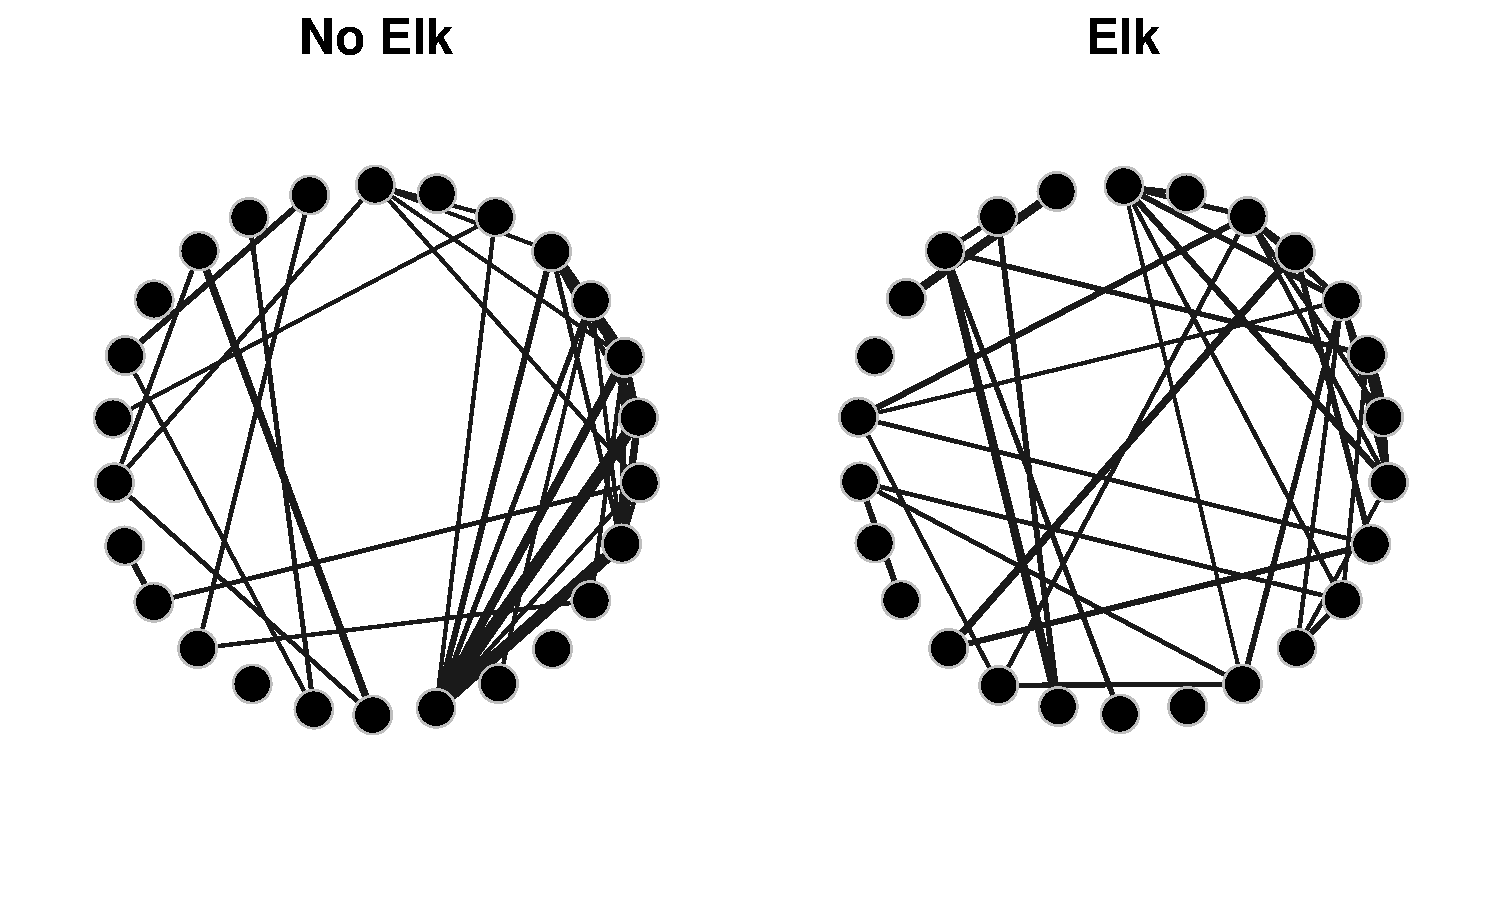
\includegraphics{SPN_figures-net1}
\end{center} 
\caption{Network graph for elk and no elk exposed solidago offspring
  arranged in circle. Points represent species and lines represent
  statistically significant Kendall's tau correlation
  coefficients.} 
\label{fig:one}
\end{figure}

\begin{figure} 
\begin{center} 
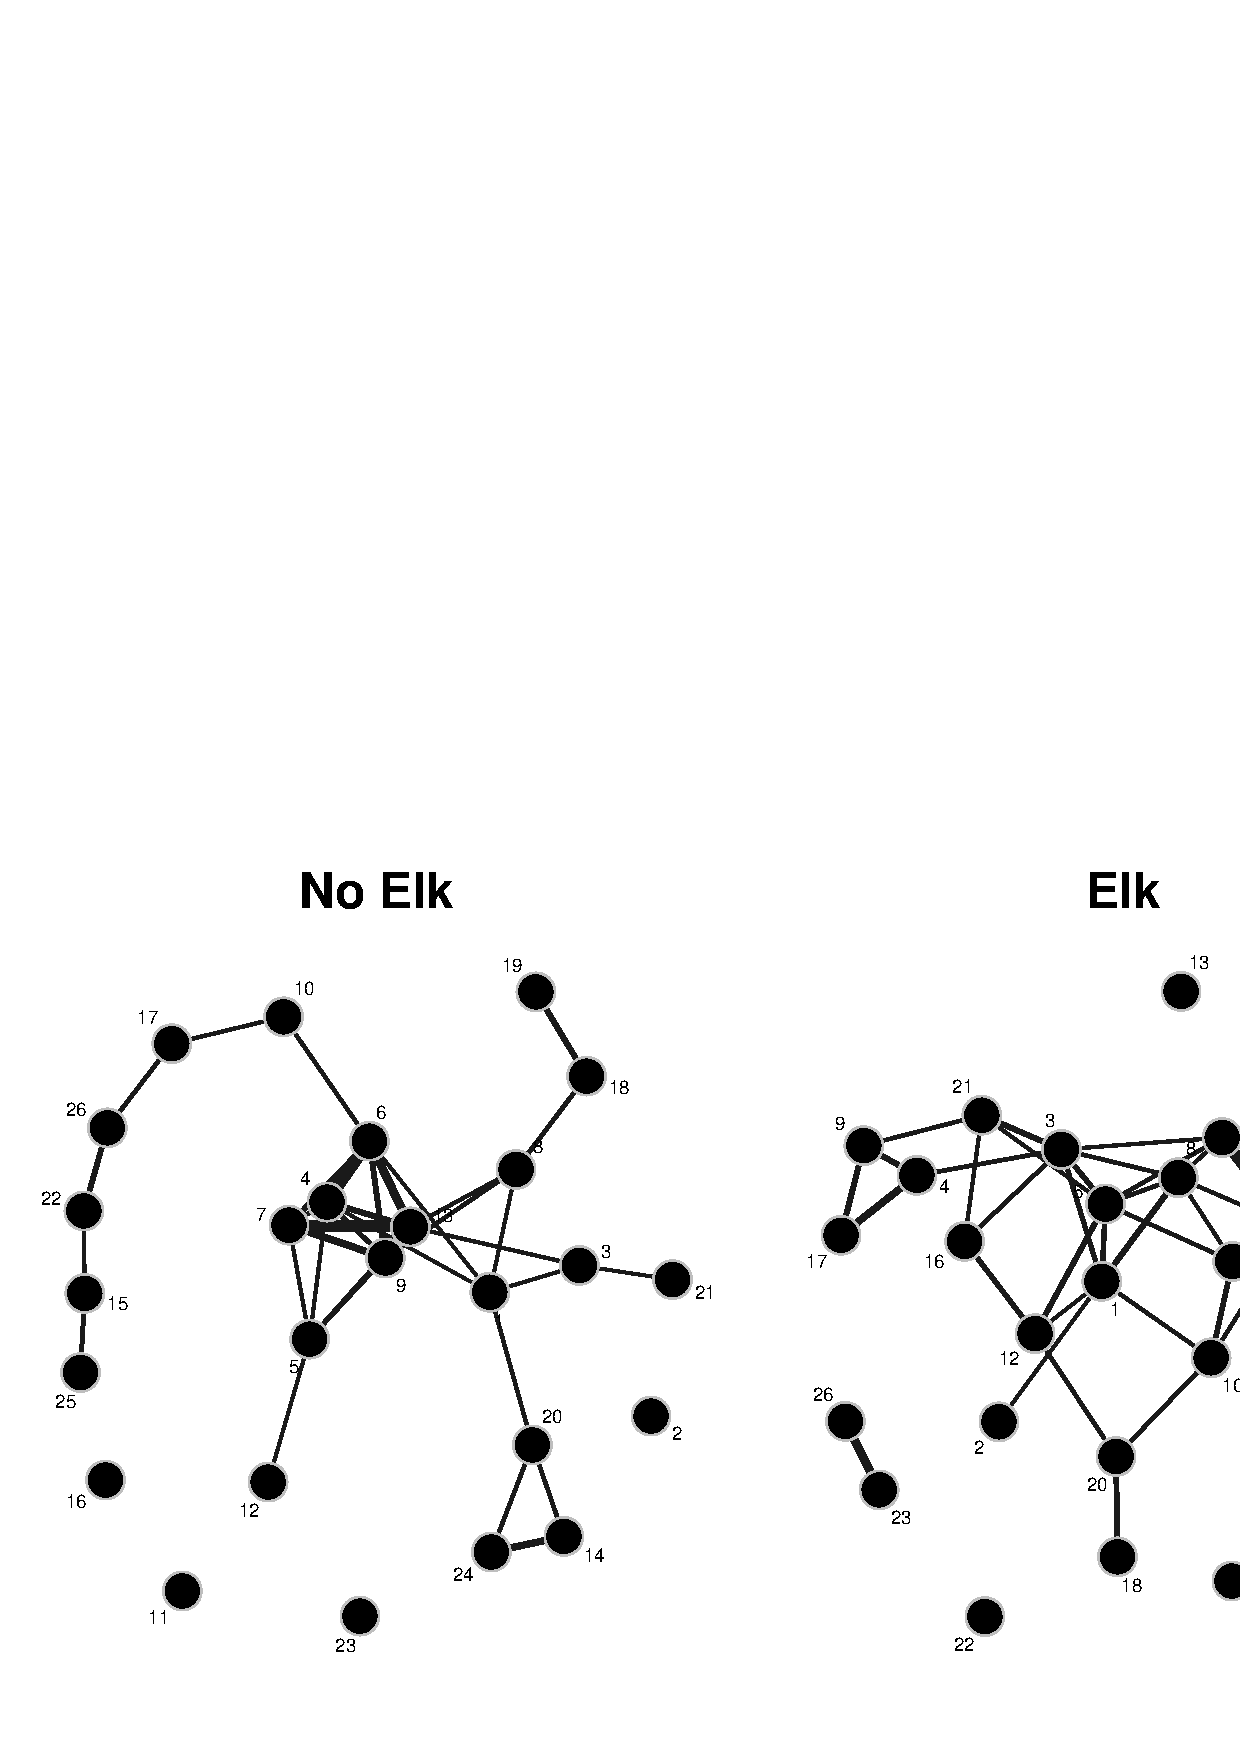
\includegraphics{SPN_figures-net2}
\end{center} 
\caption{Network graph for elk and no elk exposed solidago offspring
  arranged using a physical force algorithm. Points represent species and lines represent
  statistically significant Kendall's tau correlation
  coefficients.} 
\label{fig:two}
\end{figure}

\subsection*{Corresponding Species Labels}
\begin{Schunk}
\begin{Soutput}
 [1] "Grey.Beetle = 1"           "Aphid = 2"                
 [3] "Ant = 3"                   "BlackOrangeWasp = 4"      
 [5] "Syrphid.Fly = 5"           "RedBlackFly = 6"          
 [7] "LargeHairyFly = 7"         "Tiny.Fly = 8"             
 [9] "GreenTrueBug = 9"          "SkinnyBlackFly = 10"      
[11] "BlackYellowFly = 11"       "BrightGreenFly = 12"      
[13] "GreyMoth = 13"             "BlackWasp = 14"           
[15] "Wasp = 15"                 "HumpbackFly = 16"         
[17] "Thrips = 17"               "SkinnyBee = 18"           
[19] "BrownFly = 19"             "HoneyBee = 20"            
[21] "BigBlackFly = 21"          "BlackGreyFly = 22"        
[23] "Microbutterfly = 23"       "LongHornBeetle = 24"      
[25] "BlackWhiteFly = 25"        "OrangeYellowHairyBee = 26"
\end{Soutput}
\end{Schunk}

\subsection*{Network Structural Statistics}
\begin{Schunk}
\begin{Sinput}
> L <- unlist(lapply(net.list, function(x) bin.sum(x)/2))
> L
\end{Sinput}
\begin{Soutput}
No Elk    Elk 
    35     38 
\end{Soutput}
\begin{Sinput}
> unlist(lapply(net.list, function(x) centralization(x, degree)))
\end{Sinput}
\begin{Soutput}
    No Elk        Elk 
0.09895807 0.04954227 
\end{Soutput}
\begin{Sinput}
> unlist(lapply(net.list, fragmentation))
\end{Sinput}
\begin{Soutput}
   No Elk       Elk 
0.2892308 0.3507692 
\end{Soutput}
\begin{Sinput}
> ptc <- sort(apply(abs(net.list[[1]] - net.list[[2]]), 1, sum), 
+     decreasing = TRUE)/sum(apply(abs(net.list[[1]] - net.list[[2]]), 
+     1, sum)) * 100
> ptc
\end{Sinput}
\begin{Soutput}
            GreyMoth         GreenTrueBug          RedBlackFly 
           8.5564099            7.6639446            7.3241704 
     BlackOrangeWasp          Syrphid.Fly        LargeHairyFly 
           7.1767130            6.5168884            6.1632590 
            Tiny.Fly                  Ant          Grey.Beetle 
           5.6600643            5.2391345            5.0294040 
            HoneyBee       LongHornBeetle               Thrips 
           4.5365880            4.4610636            3.7685182 
OrangeYellowHairyBee       SkinnyBlackFly            SkinnyBee 
           3.3159858            2.9539405            2.8719922 
      BrightGreenFly          BigBlackFly                 Wasp 
           2.6241726            2.4213050            2.3077912 
         HumpbackFly       BlackYellowFly         BlackGreyFly 
           2.2338768            2.1914097            1.6024119 
      Microbutterfly            BlackWasp        BlackWhiteFly 
           1.5549120            1.1540013            1.1011539 
            BrownFly                Aphid 
           1.0648678            0.5060215 
\end{Soutput}
\end{Schunk}


%%QAP TEST FOR STRUCTURAL DIFFERENCES




%%QAP TEST FOR CENTRALIZATION




%% %%QAP TEST FOR FRAGMENTATION
%% %%I can't figure out why this isn't working.
%% <<echo=false,results=hide>>=
%% if (QAP == TRUE){
%% frag.qap <- function(y,g1,g2){fragmentation(y[,,g1]) - fragmentation(y[,,g2])}
%% rm(x)
%% qap.F <- qaptest(qap.in,frag.qap,reps=5000,g1=1,g2=2)
%% }
%% @ 

\subsection*{Barplots of Network Statistics}

\begin{Schunk}
\begin{Sinput}
> barplot(L, ylab = "Number of Connections", col = 1)
\end{Sinput}
\end{Schunk}

\begin{Schunk}
\begin{Sinput}
> barplot(unlist(lapply(net.list, function(x) centralization(x, 
+     degree))), ylab = "Centralization", col = 1)
\end{Sinput}
\end{Schunk}

\begin{Schunk}
\begin{Sinput}
> barplot(unlist(lapply(net.list, fragmentation)), ylab = "Fragmentation", 
+     col = 1)
\end{Sinput}
\end{Schunk}


\begin{Schunk}
\begin{Sinput}
> barplot(ptc, las = 2, col = "black", ylab = "Percent Total Change", 
+     names = 1:length(ptc))
\end{Sinput}
\end{Schunk}

\begin{figure} 
\begin{center} 
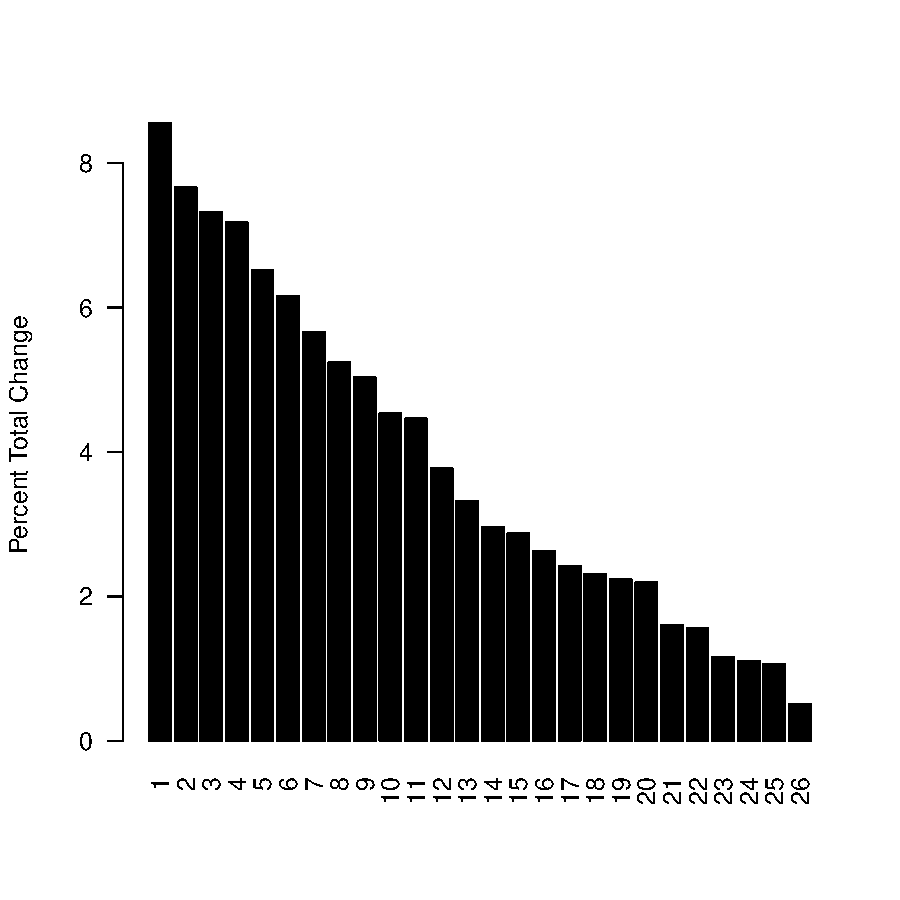
\includegraphics{SPN_figures-bpptc}
\end{center} 
\caption{Barplot of the percent total change in connections (PTC)
  comparing \textbf{Elk} and \textbf{No Elk} exposed solidago.} 
\label{fig:six}
\end{figure}

\pagebreak

\subsection*{Corresponding Species Labels for PTC Plot}
\begin{Schunk}
\begin{Soutput}
 [1] "GreyMoth"             "GreenTrueBug"         "RedBlackFly"         
 [4] "BlackOrangeWasp"      "Syrphid.Fly"          "LargeHairyFly"       
 [7] "Tiny.Fly"             "Ant"                  "Grey.Beetle"         
[10] "HoneyBee"             "LongHornBeetle"       "Thrips"              
[13] "OrangeYellowHairyBee" "SkinnyBlackFly"       "SkinnyBee"           
[16] "BrightGreenFly"       "BigBlackFly"          "Wasp"                
[19] "HumpbackFly"          "BlackYellowFly"       "BlackGreyFly"        
[22] "Microbutterfly"       "BlackWasp"            "BlackWhiteFly"       
[25] "BrownFly"             "Aphid"               
\end{Soutput}
\end{Schunk}


\begin{figure} 
\begin{center} 
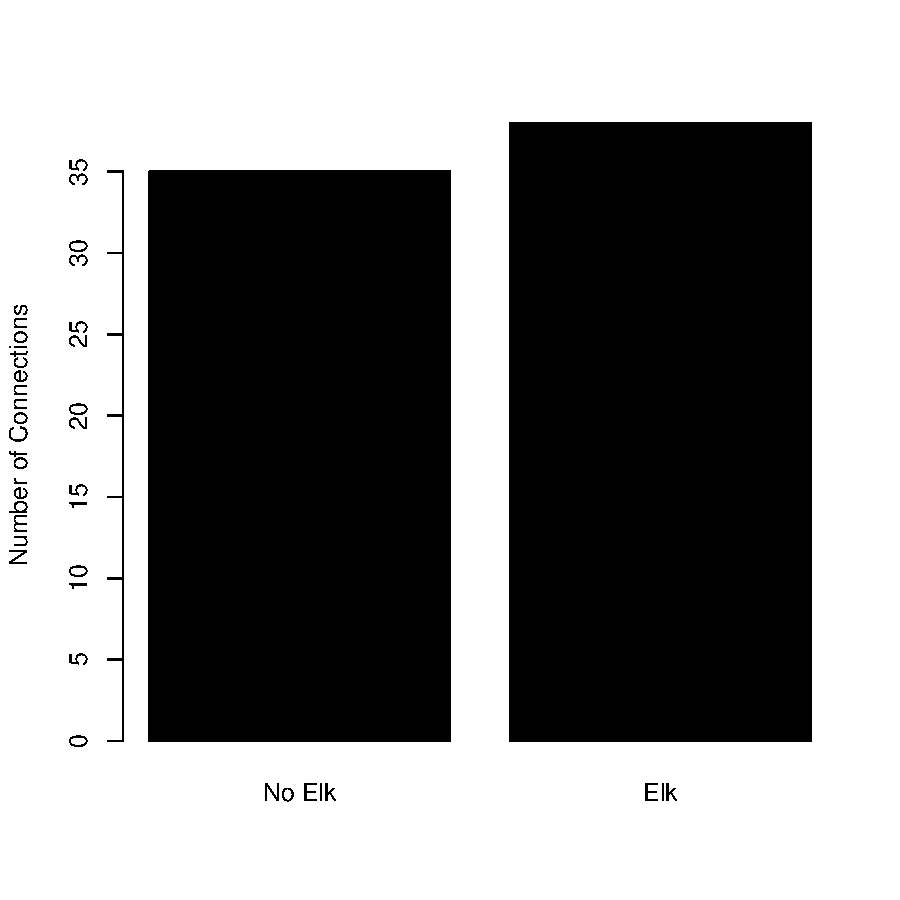
\includegraphics{SPN_figures-bpL}
\end{center} 
\caption{Barplot of the number of connetions in each graph.} 
\label{fig:three}
\end{figure}

\begin{figure} 
\begin{center} 
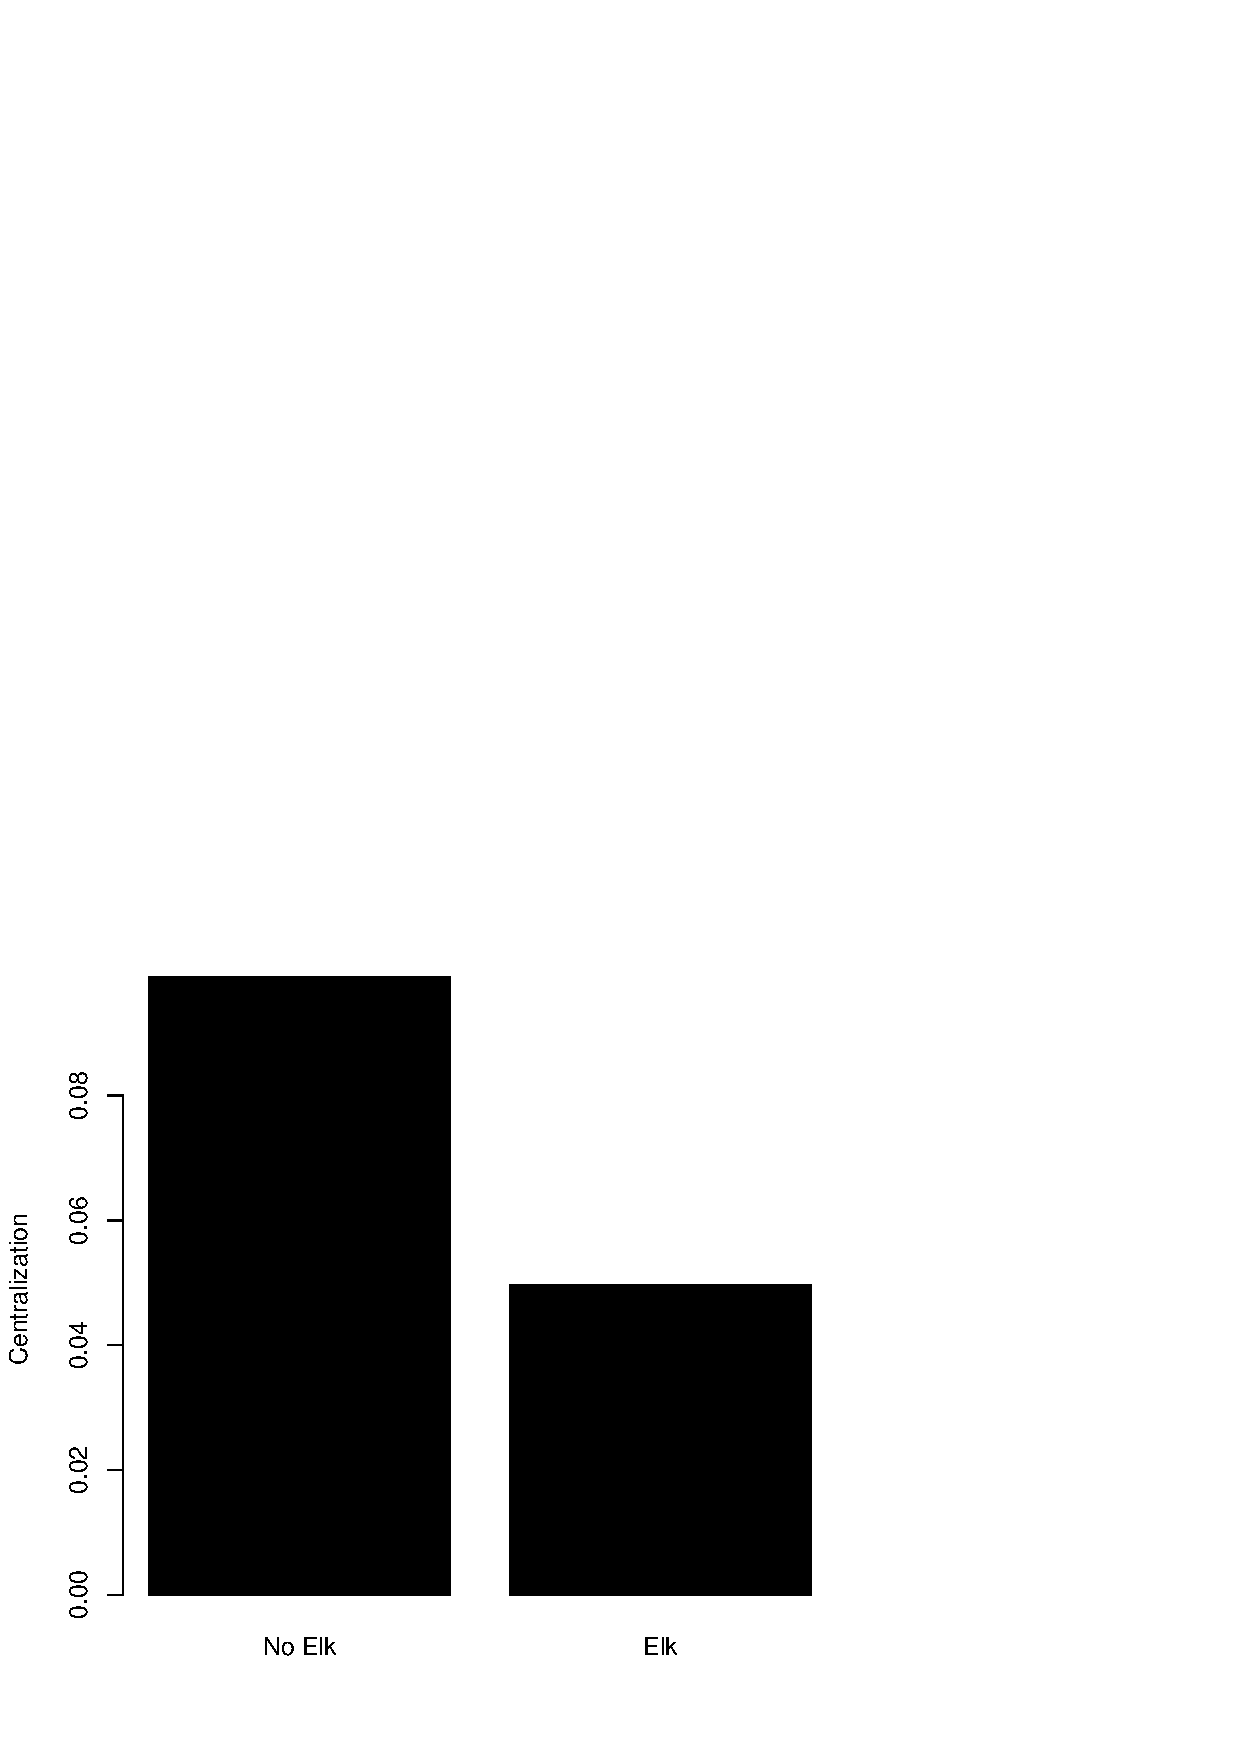
\includegraphics{SPN_figures-bpC}
\end{center} 
\caption{Barplot of the centralization of each graph.} 
\label{fig:four}
\end{figure}

\begin{figure} 
\begin{center} 
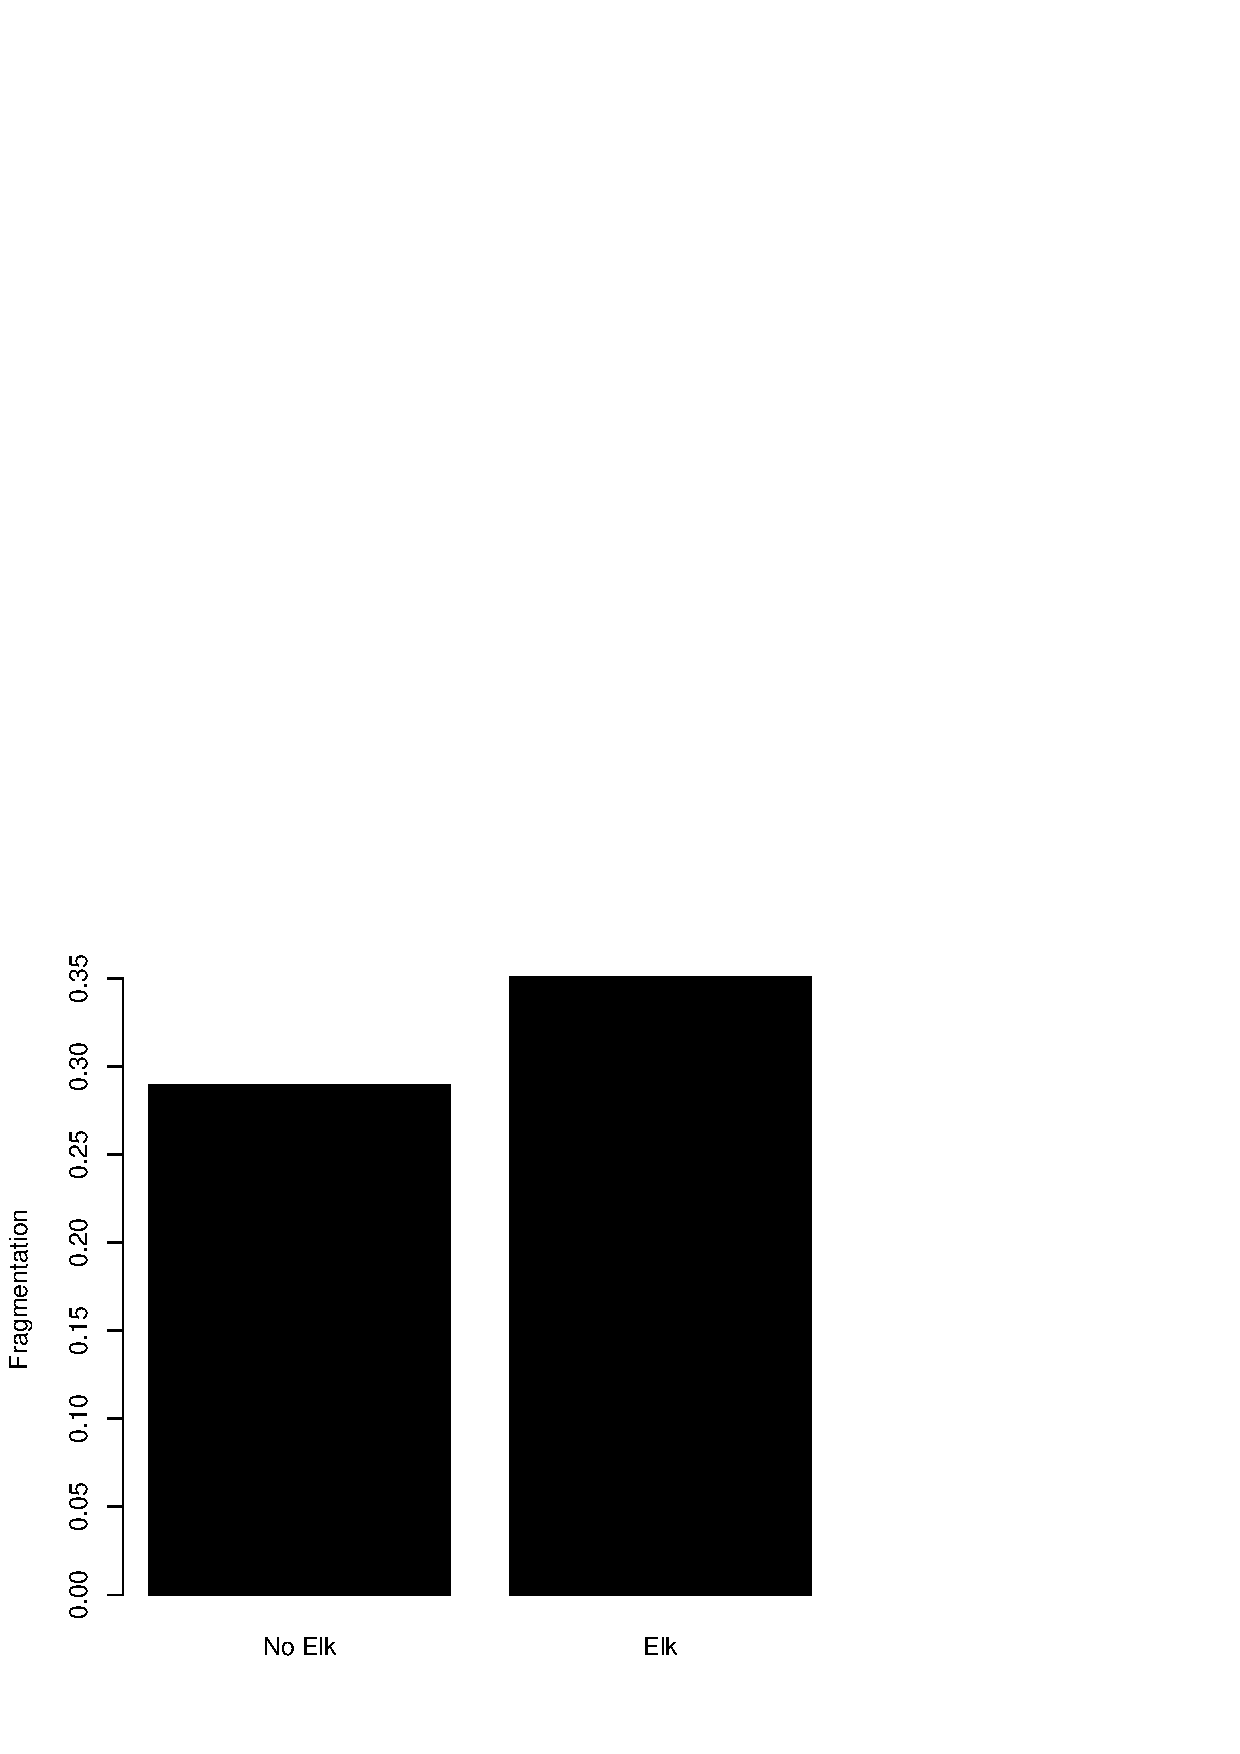
\includegraphics{SPN_figures-bpF}
\end{center} 
\caption{Barplot of the fragmentation of each graph.} 
\label{fig:five}
\end{figure}



%% <<fig=true>>=
%% barplot(ptc,las=2,col='black',ylab='Percent Total Change')
%% @ 


%% ###Use family
%% ##remove families that were replicated less than 4 times

%% com.list <- list()
%% for (i in (1:length(unique(fam)))){
%% if (nrow(com[fam == unique(fam)[i],]) <= 7){
%% }else{
%%   com.list[[i]] <- com[fam == unique(fam)[i],]
%%   names(com.list)[i] <- as.character(unique(fam)[i])
%% }
%% }

%% com.list <- com.list[names(com.list) != ""] #remove families with observations less than 4

%% net.list <- lapply(com.list,kendall.pairs,adj.method='fdr',p.adj=FALSE,alpha=0.05)
%% table(unlist(net.list))

%% ##Graphs for presenation
%% quartz('',22,11.5)
%% par(mfrow=c(2,4),mar=c(2.4,1.3,1.3,1.3),oma=c(0.1,0.1,0.1,0.1),bg='transparent',col.main='white',cex=2,mar=c(2,1,1,1))
%%                                         #names(net.list)=c('No Elk','Elk') #rename the network graphs
%% net.list.reorder <- net.list
%% com.list.reorder <- com.list
%% for (i in (1:length(net.list))){
%%       v.col=apply(com.list.reorder[[i]],2,sum); v.col[v.col != 0] = 'lightblue' #color the present species
%%             v.col[v.col == 0] <- 'black' #color empty species
%%             gplot(abs(net.list.reorder[[i]]),gmode='graph',vertex.cex=3,vertex.sides=100,vertex.col=v.col,edge.lwd=0.35,edge.col=gray(0.9)[1],vertex.border='grey',mode='circle',displaylabels=FALSE,cex=2,main=names(net.list.reorder)[i]) #without titles
%%     }


%% ##Community Analyses
%% adonis(com.~(pop/fam))

%% ##relativize by species max
%% com.sm = apply(com.,2,function(x) x/max(x))
%% adonis(com.sm~pop/fam)

%% ##relativize by site total
%% com.st = t(apply(com.,1,function(x) x/sum(x)))
%% rownames(com.st) = rownames(com.)
%% adonis(com.st~pop/fam)

%% ##presence absence data
%% com..=com.; com..[com..!=0]=1
%% adonis(com..~pop/fam)

%% colnames(data)

%% ##ordination
%% d = vegdist(com.)
%% nms = nmds(d,2,3,nits=10)
%% nms. = nmds.min(nms,2)

%% plot(nms.,col=as.numeric(pop))
%% plot(nms.,col=as.numeric(elk))

%% ##bipartite graph of whole garden

%% rs = apply(com,1,bin.sum) #row connection sum
%% cs = apply(com,2,bin.sum) #col connection sum

%% com... = com[order(rs,decreasing=TRUE),order(cs,decreasing=TRUE)] #re-order based on the species abundances and total abundance of arthropods on individuals

%% fam... = fam[order(rs,decreasing=TRUE)]
%% pop... = pop[order(rs,decreasing=TRUE)]

%% fam.col = rainbow(length(unique(as.numeric(fam...))))[as.numeric(fam...)]
%% pop.col = rainbow(length(unique(as.numeric(pop...))))[as.numeric(pop...)]

%% par(mfrow=c(2,1))
%% plotweb(com...,method='normal',col.low=fam.col,bor.col.low=fam.col,low.lablength=0,text.rot=90)
%% plotweb(com...,method='normal',col.low=pop.col,bor.col.low=pop.col,low.lablength=0,text.rot=90)


%% ##remove the aphid

%% .com = com...[,colnames(com...)!='Aphid']
%% rs = apply(.com,1,bin.sum) #row connection sum
%% cs = apply(.com,2,bin.sum) #col connection sum
%% .com = .com[order(rs,decreasing=TRUE),order(cs,decreasing=TRUE)] #re-order based on the species abundances and total abundance of arthropods on individuals

%% plotweb(.com,method='normal',col.low=rainbow(length(unique(as.numeric(fam))))[as.numeric(fam)],bor.col.low=rainbow(length(unique(as.numeric(fam))))[as.numeric(fam)],low.lablength=0)
%% plotweb(.com,method='normal',col.low=rainbow(length(unique(as.numeric(pop))))[as.numeric(pop)],bor.col.low=rainbow(length(unique(as.numeric(pop))))[as.numeric(pop)],low.lablength=0)


\end{document}  
